\باب{مفید معلومات}\شناخت{ضمیمہ_مفید_معلومات}
\حصہ{اعلی تفاعل کے مساوات}

%===============================================
\اصطلاح{قوت نمائی تفاعل} \عددی{e^x} (شکل \حوالہ{شکل_ضمیمہ_مفید_قوت_نمائی}-الف)
\begin{align*}
e=\num{2.718281828459045235360287471353}
\end{align*}
%
\begin{align}\label{مساوات_ضمیمہ_مفید_قوت_نمائی}
e^xe^y=e^{x+y},\quad \frac{e^x}{e^y}=e^{x-y},\quad (e^x)^y=e^{xy}
\end{align}

\اصطلاح{قدرتی لوگارتھم} (شکل \حوالہ{شکل_ضمیمہ_مفید_قوت_نمائی}-ب)
\begin{align}
\ln(xy)=\ln x+\ln y,\quad \ln\frac{x}{y}=\ln x-\ln y,\quad \ln(x^a)=a\ln x
\end{align}
\عددی{e^x} کا الٹ \عددی{\ln x} ہے۔اس کے علاوہ \عددی{e^{\ln x}=x} اور \عددی{e^{-\ln x}=e^{\ln{\tfrac{1}{x}}}=\tfrac{1}{x}} ہیں۔
%
\begin{figure}
\centering
\begin{subfigure}{0.5\textwidth}
\centering
\begin{tikzpicture}
\begin{axis}[small,axis lines*=middle,xlabel={$x$},ylabel={$y$},xtick={-2,-1,0,1,2,3},ytick={1,2,3,4,5,6,7},xticklabels={$-2$,{},$0$,{},$2$,{}},yticklabels={{},{},{},{},$5$,{},{}},ymin=0,ymax=7.5,xmin=-2.5,xmax=3.9,xlabel style={at={(current axis.right of origin)},anchor=north west}, ylabel style={at={(current axis.above origin)},anchor=north west},ylabel style={rotate=-90}]
\addplot[domain=-2.5:2]{e^x};
\end{axis}
\end{tikzpicture}
\caption*{(الف) قوت نمائی تفاعل \عددی{e^x}}
\end{subfigure}%
\begin{subfigure}{0.5\textwidth}
\centering
\begin{tikzpicture}
\begin{axis}[small,axis lines*=middle,xlabel={$x$},ylabel={$y$},xtick={1,2,3,4,5,6,7,8,9,10},xticklabels={{},{},{},{},{$5$},{},{},{},{},{$10$}},ytick={-2,-1,0,1,2,3,4},yticklabels={{$-2$},{},{$0$},{},{$2$},{},{}},ymin=-2.5,ymax=5.9,xmin=0,xmax=10.5,xlabel style={at={(current axis.right of origin)},anchor=north west}, ylabel style={at={(current axis.above origin)},anchor=north west},ylabel style={rotate=-90}]
\addplot[domain=0:10,samples=100]{ln(x)};
\end{axis}
\end{tikzpicture}
\caption*{(ب) قدرتی لوگارتھم \عددی{\ln x}}
\end{subfigure}%
\caption{قوت نمائی تفاعل اور قدرتی لوگارتھم تفاعل}
\label{شکل_ضمیمہ_مفید_قوت_نمائی}
\end{figure}
%==================================

\اصطلاح{اساس دس کا لوگارتھم} \عددی{\log_{10}x} یا \عددی{\log x}
\begin{align}
\log x&=M\ln x,\quad M=\log e=\num{0.434294481903251827651128918917}\\
\ln x&=\frac{1}{M}\log x, \quad \frac{1}{M}=\num{2.302585092994045684017991454684}
\end{align}
\عددی{10^x} کا الٹ \عددی{\log x} ہے۔اس کے علاوہ \عددی{10^{\log x}=x} اور \عددی{10^{-\log x}=10^{\log \tfrac{1}{x}}=\tfrac{1}{x}} ہیں۔
%==========================================

\اصطلاح{سائن اور کوسائن تفاعل} (شکل \حوالہ{شکل_ضمیمہ_مفید_سائن_نما}-الف اور ب)۔ احصائے تکملات میں زاویہ کو ریڈئیں میں ناپا جاتا ہے۔یوں \عددی{\sin x} اور \عددی{\cos x} کا دوری عرصہ \عددی{2\pi} ہو گا۔\عددی{\sin x} طاق ہے یعنی \عددی{\sin (-x)=-\sin x} ہو گا جبکہ \عددی{\cos x} جفت ہے یعنی \عددی{\cos(-x)=\cos x} ہو گا۔
\begin{figure}
\centering
\begin{subfigure}{0.5\textwidth}
\centering
\begin{tikzpicture}
\begin{axis}[small,axis lines*=middle,xlabel={$x$},ylabel={$y$},xtick={-90,90,180,270,360,450},xticklabels={{},{},{$\pi$},{},{$2\pi$},{}},ytick={-1,1},yticklabels={{$-1$},{$1$}},xlabel style={at={(current axis.right of origin)},anchor=north east},ylabel style={rotate=-90},ylabel style={at={(current axis.above origin)},anchor=north east},ymin=-2,ymax=2]
\addplot[domain=-90:500,samples=100]{sin(x)};
\end{axis}
\end{tikzpicture}
\caption*{(الف) \عددی{\sin x}}
\end{subfigure}%
\begin{subfigure}{0.5\textwidth}
\centering
\begin{tikzpicture}
\begin{axis}[small,axis lines*=middle,xlabel={$x$},ylabel={$y$},xtick={-90,90,180,270,360,450},xticklabels={{},{},{$\pi$},{},{$2\pi$},{}},ytick={-1,1},yticklabels={{$-1$},{$1$}},xlabel style={at={(current axis.right of origin)},anchor=north east},ylabel style={rotate=-90},ylabel style={at={(current axis.above origin)},anchor=north east},ymin=-2,ymax=2]
\addplot[domain=-90:500,samples=100]{cos(x)};
\end{axis}
\end{tikzpicture}
\caption*{(ب) \عددی{\cos x}}
\end{subfigure}%
\caption{سائن نما تفاعل}
\label{شکل_ضمیمہ_مفید_سائن_نما}
\end{figure}
%
\begin{align*}
1^{\circ}=&\SI{0.017453292519943}{\radian}\\
\SI{1}{radian}&=57^\circ\,17'\,44.80625"=57.2957795131^{\circ}
\end{align*}
%
\begin{align}
\sin^2x+\cos^2x=1
\end{align}
%
\begin{gather}
\begin{aligned}
\sin(x-y)&=\sin x\cos y-\cos x\sin y\\
\cos(x+y)&=\cos x\cos y-\sin x\sin y\\
\cos(x-y)&=\cos x\cos y+\sin x\sin y
\end{aligned}
\end{gather}
%
\begin{align}
\sin 2x=2\sin x\cos x, \quad \cos 2x=\cos^2x-\sin^2x
\end{align}
%
\begin{gather}
\begin{aligned}
\sin x&=\cos\left(x-\frac{\pi}{2}\right)=\cos\left(\frac{\pi}{2}-x\right)\\
\cos x&=\sin\left(x+\frac{\pi}{2}\right)=\sin\left(\frac{\pi}{2}-x\right)
\end{aligned}
\end{gather}
%
\begin{align}
\sin(\pi-x)&=\sin x,\quad \cos(\pi-x)=-\cos x\\
\cos^2x&=\frac{1}{2}(1+\cos 2x),\quad \sin^2x=\frac{1}{2}(1-\cos 2x)
\end{align}
%
\begin{gather}
\begin{aligned}\label{مساوات_ضمیمہ_مفید_گیارہ}
\sin x\sin y&=\frac{1}{2}[-\cos(x+y)+\cos(x-y)]\\
\cos x\cos y&=\frac{1}{2}[\cos(x+y)+\cos(x-y)]\\
\sin x\cos y&=\frac{1}{2}[\sin(x+y)+\sin(x-y)]
\end{aligned}
\end{gather}
%
\begin{gather}
\begin{aligned}
\sin u+\sin v&=2\sin \frac{u+v}{2}\cos\frac{u-v}{2}\\
\cos u+\cos v&=2\cos\frac{u+v}{2}\cos\frac{u-v}{2}\\
\cos v-\cos u&=2\sin\frac{u+v}{2}\sin\frac{u-v}{2}
\end{aligned}
\end{gather}
%
\begin{align}
A\cos x+B\sin x&=\sqrt{A^2+B^2}\cos(x\mp\delta),\quad \tan \delta=\frac{\sin \delta}{\cos \delta}=\pm \frac{B}{A}\\
A\cos x+B\sin x &=\sqrt{A^2+B^2}\sin(x\mp\delta),\quad \tan \delta=\frac{\sin \delta}{\cos \delta}=\mp\frac{A}{B}
\end{align}
\اصطلاح{ٹینجنٹ، کوٹینجنٹ، سیکنٹ، کوسیکنٹ} (شکل \حوالہ{شکل_ضمیمہ_مفید_ٹینجنٹ_کوٹینجنٹ}-الف، ب)
\begin{align}
\tan x&=\frac{\sin x}{\cos x}\, ,\quad \cot x=\frac{\cos x}{\sin x}\, ,\quad \sec x=\frac{1}{\cos x}\, ,\quad \csc=\frac{1}{\sin x}\\
\tan(x+y)&=\frac{\tan x+\tan y}{1-\tan x\tan y},\quad \tan(x-y)=\frac{\tan x-\tan y}{1+\tan x\tan y}
\end{align}
%
\begin{figure}
\centering
\begin{subfigure}{0.5\textwidth}
\centering
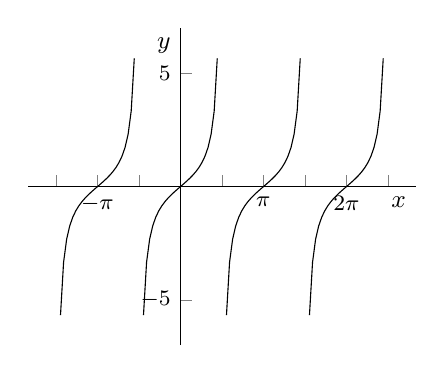
\begin{tikzpicture}
\begin{axis}[small,axis lines*=middle,xlabel={$x$},ylabel={$y$},xlabel style={at={(current axis.right of origin)},anchor=north east},ylabel style={rotate=-90},ylabel style={at={(current axis.above origin)},anchor=north east},ymin=-7,ymax=7,xtick={-270,-180,-90,90,180,270,360,450,540},xticklabels={{},{$-\pi$},{},{},{$\pi$},{},{$2\pi$},{},{}},ytick={-5,5},yticklabels={{$-5$},{$5$}}]
\addplot[domain=-260:-100]{tan(x)};
\addplot[domain=-80:80]{tan(x)};
\addplot[domain=100:260]{tan(x)};
\addplot[domain=280:440]{tan(x)};
\end{axis}
\end{tikzpicture}
\caption*{(الف) \عددی{\tan x}}
\end{subfigure}%
\begin{subfigure}{0.5\textwidth}
\centering
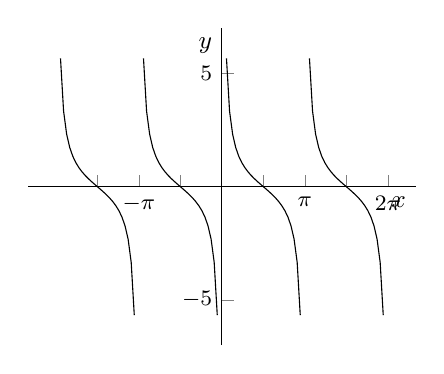
\begin{tikzpicture}
\begin{axis}[small,axis lines*=middle,xlabel={$x$},ylabel={$y$},xlabel style={at={(current axis.right of origin)},anchor=north east},ylabel style={rotate=-90},ylabel style={at={(current axis.above origin)},anchor=north east},ymin=-7,ymax=7,xtick={-270,-180,-90,90,180,270,360,450,540},xticklabels={{},{$-\pi$},{},{},{$\pi$},{},{$2\pi$},{},{}},ytick={-5,5},yticklabels={{$-5$},{$5$}}]
\addplot[domain=-350:-190]{cot(x)};
\addplot[domain=-170:-10]{cot(x)};
\addplot[domain=10:170]{cot(x)};
\addplot[domain=190:350]{cot(x)};
\end{axis}
\end{tikzpicture}
\caption*{(ب) \عددی{\cot x}}
\end{subfigure}%
\caption{ٹینجنٹ اور کوٹینجنٹ}
\label{شکل_ضمیمہ_مفید_ٹینجنٹ_کوٹینجنٹ}
\end{figure}
%========================
\اصطلاح{ہذلولی تفاعل} (ہذلولی سائن \عددی{\sin h x} وغیرہ۔ شکل \حوالہ{شکل_ضمیمہ_مفید_ہذلولی_تفاعل}-الف، ب)
\begin{align}
\sinh x&=\frac{1}{2}(e^x-e^{-x}),\quad \cosh x=\frac{1}{2}(e^x+e^{-x})\\
\tanh x&=\frac{\sinh x}{\cosh x}\, ,\quad \coth x=\frac{\cosh x}{\sinh x}\\
\cosh x+\sinh x&=e^x,\quad \cosh x-\sinh x=e^{-x}
\end{align}
%
\begin{align}
\cosh^2 x-\sinh^2 x&=1
\end{align}
%
\begin{align}
\sinh^2=\frac{1}{2}(\cosh 2x-1),\quad \cosh^2 x=\frac{1}{2}(\cosh 2x+1)
\end{align}
%==================================
\begin{gather}
\begin{aligned}
\sinh(x\mp y)&=\sinh x\cosh y\mp \cosh x\sinh y\\
\cosh(x\mp y)&=\cosh x\cosh y\mp \sinh x\sinh y
\end{aligned}
\end{gather}
%
\begin{align}
\tanh(x\mp y)=\frac{\tanh x\mp \tanh y}{1\mp \tanh x\tanh y}
\end{align}
%
\begin{figure}
\centering
\begin{subfigure}{0.5\textwidth}
\centering
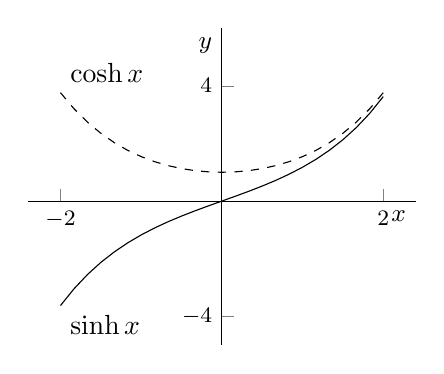
\begin{tikzpicture}
\begin{axis}[small,axis lines*=middle,xlabel={$x$},ylabel={$y$},xlabel style={at={(current axis.right of origin)},anchor=north east},ylabel style={rotate=-90},ylabel style={at={(current axis.above origin)},anchor=north east},ymin=-5,ymax=6,xtick={-2,2},xticklabels={{$-2$},{$2$}},ytick={-4,4},yticklabels={{$-4$},{$4$}}]
\addplot[domain=-2:2]{sinh(x)}node[pos=0,below right]{$\sinh x$};
\addplot[dashed,domain=-2:2]{cosh(x)}node[pos=0,above right]{$\cosh x$};
\end{axis}
\end{tikzpicture}
\caption*{(الف) ٹھوس خط \عددی{\sinh x} ہے جبکہ نقطہ دار خط \عددی{\cosh x} ہے۔}
\end{subfigure}%
\begin{subfigure}{0.5\textwidth}
\centering
\begin{tikzpicture}
\begin{axis}[small,axis lines*=middle,xlabel={$x$},ylabel={$y$},xlabel style={at={(current axis.right of origin)},anchor=north east},ylabel style={rotate=-90},ylabel style={at={(current axis.above origin)},anchor=north east},ymin=-5,ymax=6,xtick={-2,2},xticklabels={{$-2$},{$2$}},ytick={-4,4},yticklabels={{$-4$},{$4$}}]
\addplot[domain=-2:2]{tanh(x)};
\addplot[dashed,domain=0.2:2]{1/tanh(x)};
\addplot[dashed,domain=-2:-0.2]{1/tanh(x)};
\end{axis}
\end{tikzpicture}
\caption*{(ب) ٹھوس خط \عددی{\tanh x} ہے جبکہ نقطہ دار خط \عددی{\coth x} ہے۔}
\end{subfigure}%
\caption{ہذلولی سائن، ہذلولی تفاعل۔}
\label{شکل_ضمیمہ_مفید_ہذلولی_تفاعل}
\end{figure}
%====================
\اصطلاح{گیما تفاعل} (شکل \حوالہ{شکل_ضمیمہ_مفید_گیما_تفاعل}) \عددی{\Gamma(\alpha)} کی تعریف درج ذیل تکمل ہے
\begin{align}\label{مساوات_ضمیمہ_گیما_تکمل_الف}
\Gamma(\alpha)=\int_{0}^{\infty} e^{-t}t^{\alpha-1}\dif t \quad \quad (\alpha>0)
\end{align}
جو صرف مثبت (\عددی{\alpha > 0}) کے لئے معنی رکھتا ہے (یا اگر ہم مخلوط \عددی{\alpha} کی بات کریں تب یہ \عددی{\alpha} کی ان قیمتوں کے لئے معنی رکھتا ہے جن  کا حقیقی جزو مثبت ہو)۔تکمل بالحصص سے درج ذیل اہم تعلق حاصل ہوتا ہے۔
\begin{align}\label{مساوات_ضمیمہ_گیما_تکمل_ب}
\Gamma(\alpha+1)=\alpha\Gamma(\alpha)
\end{align}
مساوات \حوالہ{مساوات_ضمیمہ_گیما_تکمل_الف} سے \عددی{\Gamma(1)=1} ملتا ہے۔ یوں مساوات \حوالہ{مساوات_ضمیمہ_گیما_تکمل_ب} استعمال کرتے ہوئے \عددی{\Gamma(2)=1} حاصل ہو گا جسے دوبارہ مساوات \حوالہ{مساوات_ضمیمہ_گیما_تکمل_ب} میں استعمال کرتے ہوئے \عددی{\Gamma(3)=2\times 1} ملتا ہے۔اسی طرح بار بار مساوات \حوالہ{مساوات_ضمیمہ_گیما_تکمل_ب} استعمال کرتے ہوئے \عددی{\alpha} کی کسی بھی عدد صحیح مثبت قیمت \عددی{k} کے لئے درج ذیل حاصل ہوتا ہے۔
\begin{align}\label{مساوات_ضمیمہ_گیما_تکمل_پ}
\Gamma(k+1)=k!\quad \quad (k=0,1,2,\cdots)
\end{align} 
مساوات \حوالہ{مساوات_ضمیمہ_گیما_تکمل_ب} کے بار بار استعمال سے  درج ذیل حاصل ہوتا ہے
\begin{align*}
\Gamma(\alpha)=\frac{\Gamma(\alpha+1)}{\alpha}=\frac{\Gamma(\alpha+2)}{\alpha(\alpha+1)}=\cdots=\frac{\Gamma(\alpha+k+1)}{\alpha(\alpha+1)(\alpha+2)\cdots(\alpha+k)}
\end{align*}
جس کو استعمال کرتے ہوئے ہم \عددی{\alpha} کی منفی قیمتوں کے لئے گیما تفاعل کی درج ذیل تعریف پیش کرتے ہیں
\begin{align}\label{مساوات_ضمیمہ_گیما_تکمل_ت}
\Gamma(\alpha)=\frac{\Gamma(\alpha+k+1)}{\alpha(\alpha+1)(\alpha+2)\cdots(\alpha+k)}\quad \quad (\alpha\ne 0, -1,-2,\cdots)
\end{align}
جہاں \عددی{k} کی ایسی کم سے کم قیمت چنی جاتی ہے کہ \عددی{\alpha+k+1>0} ہو۔مساوات \حوالہ{مساوات_ضمیمہ_گیما_تکمل_الف} اور مساوات \حوالہ{مساوات_ضمیمہ_گیما_تکمل_ت} مل کر \عددی{\alpha} کی تمام مثبت قیمتوں اور غیر عددی صحیحی منفی قیمتوں کے لئے گیما تفاعل دیتے ہیں۔

گیما تفاعل کو حاصل ضرب کی حد بھی فرض کیا جا سکتا ہے یعنی
\begin{align}\label{مساوات_ضمیمہ_گیما_تکمل_ٹ}
\Gamma(\alpha)=\lim_{n\to \infty} \frac{n! n^{\alpha}}{\alpha(\alpha+1)(\alpha+2)\cdots(\alpha+n)} \quad \quad (\alpha \ne 0, -1,\cdots)
\end{align}  
مساوات \حوالہ{مساوات_ضمیمہ_گیما_تکمل_ت} اور مساوات \حوالہ{مساوات_ضمیمہ_گیما_تکمل_ٹ} سے ظاہر ہے کہ مخلوط \عددی{\alpha} کی صورت میں \عددی{\alpha=0,-1,-2,\cdots} پر گیما تفاعل کے قطب پائے جاتے ہیں۔

\عددی{\alpha} کی بڑی قیمت کے لئے گیما تفاعل کی قیمت کو درج ذیل\اصطلاح{کلیہ سٹرلنگ} سے حاصل کیا جا سکتا ہے جہاں \عددی{e} قدرتی لوگارتھم کی اساس ہے۔
\begin{align}
\Gamma(\alpha+1)\approx \sqrt{2\pi \alpha}\left(\frac{\alpha}{e}\right)^\alpha
\end{align}
آخر میں گیما تفاعل کی ایک اہم اور مخصوص (درج ذیل) قیمت کا ذکر کرتے ہیں۔
\begin{align}
\Gamma\left(\frac{1}{2}\right)=\sqrt{\pi}
\end{align}
%
\begin{figure}
\centering
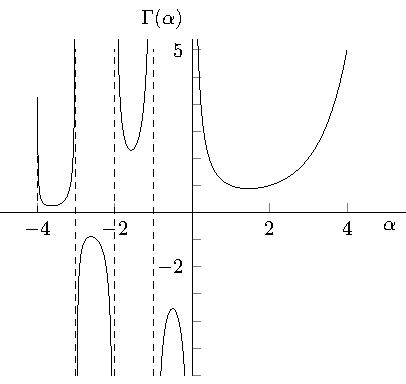
\includegraphics{figOctaveGammaFunction}
\caption{گیما تفاعل}
\label{شکل_ضمیمہ_مفید_گیما_تفاعل}
\end{figure}
%

\اصطلاح{نا مکمل گیما تفاعل}
\begin{align}
P(\alpha,x)=\int_{0}^{x} e^{-t}t^{\alpha-1}\dif t, \quad Q(\alpha,x)=\int_{x}^{\infty} e^{-t}t^{\alpha-1}\dif t \quad \quad (\alpha>0)
\end{align}
%
\begin{align}
\Gamma(\alpha)=P(\alpha,x)+Q(\alpha,x)
\end{align}
\اصطلاح{بیٹا تفاعل}
\begin{align}
B(x,y)=\int_{0}^{1}t^{x-1}(1-t)^{y-1}\dif t\quad \quad (x>0,\, y>0)
\end{align}
بیٹا تفاعل کو گیما تفاعل کی صورت میں بھی پیش کیا جا سکتا ہے۔
\begin{align}
B(x,y)=\frac{\Gamma(x) \Gamma(y)}{\Gamma(x+y)}
\end{align}
\اصطلاح{تفاعل خلل}(شکل \حوالہ{شکل_ضمیمہ_مفید_تفاعل_خلل})
\begin{align}\label{مساوات_ضمیمہ_تفاعل_خلل_الف}
\erf x=\frac{2}{\sqrt{\pi}}\int_{0}^{x} e^{-t^2}\dif t
\end{align}
مساوات \حوالہ{مساوات_ضمیمہ_تفاعل_خلل_الف} کے تفرق \عددی{\erf' x=\tfrac{2}{\sqrt{\pi}}e^{-t^2}} کی مکلارن تسلسل 
\begin{align*}
\erf' x=\frac{2}{\sqrt{\pi}}\left(x-\frac{x^3}{1!3}+\frac{x^5}{2!5}-\frac{x^7}{3!7}+-\cdots \right)
\end{align*}
 کا تکمل لینے سے تفاعل خلل کی تسلسل صورت حاصل ہوتی ہے۔
%
\begin{align}
\erf x=\frac{2}{\sqrt{\pi}}\left(x-\frac{x^3}{1!3}+\frac{x^5}{2!5}-\frac{x^7}{3!7}+-\cdots \right)
\end{align}
\عددی{erf \infty =1} ہے۔ \اصطلاح{مکملہ تفاعل خلل}
\begin{align}
\erfc x=1-\erf x=\frac{2}{\sqrt{\pi}} \int_{x}^{\infty} e^{-t^2}\dif t
\end{align}
%
\begin{figure}
\centering
\begin{tikzpicture}[
    declare function={erf(\x)=%
      (1+(e^(-(\x*\x))*(-265.057+abs(\x)*(-135.065+abs(\x)%
      *(-59.646+(-6.84727-0.777889*abs(\x))*abs(\x)))))%
      /(3.05259+abs(\x))^5)*(\x>0?1:-1);},
    declare function={erf2(\x,\y)=erf(\x)+erf(\y);}
]
\begin{axis}[small,axis lines*=middle,xlabel={$x$},ylabel={$\erf x$},xlabel style={at={(current axis.right of origin)},anchor=north east},ylabel style={rotate=-90},ylabel style={at={(current axis.above origin)},anchor=north east},ymin=-1.2,ymax=1.5,xmin=-2.2,xmax=3,xtick={-2,-1,1,2},xticklabels={{$-2$},{$-1$},{$1$},{$2$}},ytick={-1,1},yticklabels={{$-1$},{$1$}}]
\addplot[domain=-2:2]{erf(\x)};
\end{axis}
\end{tikzpicture}
\caption{تفاعل خلل۔}
\label{شکل_ضمیمہ_مفید_تفاعل_خلل}
\end{figure}
\اصطلاح{فرسنل تکملات} (شکل \حوالہ{شکل_ضمیمہ_مفید_فرسنل_تکملات})
\begin{align}
\FC(x)=\int_{0}^{x} \cos(t^2)\dif t,\quad \FS(x)=\int_{0}^{x}\sin(t^2)\dif t
\end{align}
\عددی{\FC(\infty)=\sqrt{\tfrac{\pi}{8}}} اور \عددی{\FS(\infty)=\sqrt{\tfrac{\pi}{8}}} ہیں۔\اصطلاح{مکملہ تفاعل}\حاشیہب{complementary functions}
\begin{align}
\FAC(x)&=\frac{\pi}{8}-\FC(x)=\int_{x}^{\infty} \cos(t^2)\dif t\\
\FAS(x)&=\frac{\pi}{8}-\FS(x)=\int_{x}^{\infty} \sin(t^2)\dif t
\end{align}
%
\begin{figure}
\centering
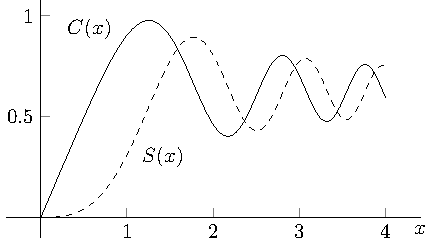
\includegraphics{figFresnelIntegrals}
\caption{فرسنل تکملات}
\label{شکل_ضمیمہ_مفید_فرسنل_تکملات}
\end{figure}
\اصطلاح{تکمل سائن} (شکل \حوالہ{شکل_ضمیمہ_مفید_تکمل_سائن})
\begin{align}
\kSi(x)=\int_{0}^{x}\frac{\sin t}{t} \dif t
\end{align}
\عددی{\kSi{\infty}=\tfrac{\pi}{2}} کے برابر ہے۔تکملہ تفاعل
\begin{align}
\ksi(x)=\frac{\pi}{2}-\kSi(x)=\int_{x}^{\infty} \frac{\sin t}{t}\dif t
\end{align}
\اصطلاح{تکمل کوسائن}
\begin{align}
\ci(x)=\int_{x}^{\infty}\frac{\cos t}{t}\dif t \quad \quad (x>0)
\end{align}
\اصطلاح{تکمل قوت نمائی}
\begin{align}
\Ei(x)=\int_{x}^{\infty} \frac{e^{-t}}{t}\dif t\quad \quad (x>0)
\end{align}
\اصطلاح{تکمل لوگارتھمی}
\begin{align}
\li(x)=\int_{0}^{x}\frac{\dif t}{\ln t}
\end{align}
%
\begin{figure}
\centering
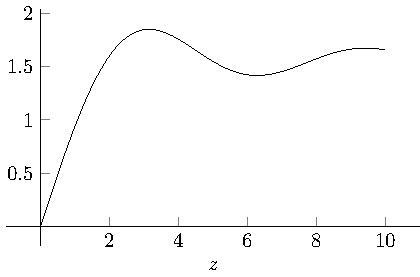
\includegraphics{figSineIntegral}
\caption{تکمل سائن}
\label{شکل_ضمیمہ_مفید_تکمل_سائن}
\end{figure}
